% 角平分线定义图：OC 平分 ∠AOB，两个角相等
\documentclass[tikz,border=4pt]{standalone}
\usepackage{ctex}
\usepackage{amsmath}
\usetikzlibrary{calc, arrows.meta, decorations.markings}
\begin{document}
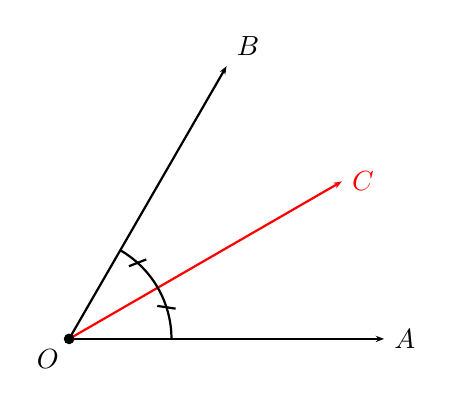
\begin{tikzpicture}[scale=1.0, thick,
  tick/.style={postaction={decorate, decoration={markings,
    mark=at position 0.6 with {\draw (-1.5pt,-3pt) -- (1.5pt,3pt);}}}}]
  \coordinate (O) at (0,0);
  \coordinate (A) at (4,0);
  \coordinate (B) at ({4*cos(60)}, {4*sin(60)});
  \coordinate (C) at ({4*cos(30)}, {4*sin(30)});
  \draw[-{Stealth[length=3pt]}] (O) -- (A);
  \draw[-{Stealth[length=3pt]}] (O) -- (B);
  \draw[-{Stealth[length=3pt]}, red] (O) -- (C);
  % 两个相等的角
  \draw[tick] (1.3,0) arc (0:30:1.3);
  \draw[tick] ({1.3*cos(30)}, {1.3*sin(30)}) arc (30:60:1.3);
  \filldraw (O) circle (1.5pt);
  \node[below left] at (O) {$O$};
  \node[right] at (A) {$A$};
  \node[above right] at (B) {$B$};
  \node[right, red] at (C) {$C$};
\end{tikzpicture}
\end{document}
